\documentclass[11pt,a4paper]{article}

% -----------------------------------------------------------------------------
% Paquetes: todos forman parte de una instalación estándar de LaTeX.
% -----------------------------------------------------------------------------
\usepackage[utf8]{inputenc}
\usepackage{enumitem}
\usepackage{float}
\usepackage{amsmath}
\usepackage{amssymb}
\usepackage{booktabs}
\usepackage[T1]{fontenc}
% Fecha en español sin depender de babel ni de spanish.ldf.
\newcommand{\FechaEnEspanol}{%
  \number\day\space de\space
  \ifcase\month
    \or enero\or febrero\or marzo\or abril\or mayo\or junio\or
    julio\or agosto\or septiembre\or octubre\or noviembre\or diciembre
  \fi\space de\space\number\year
}
\usepackage[a4paper,margin=2.5cm,headheight=42pt]{geometry}
\usepackage{graphicx}
\usepackage{xcolor}
\usepackage{fancyhdr}

% lastpage no es necesario para compilar, pero permite mostrar "página de N".
\newif\ifHayUltimaPagina
\IfFileExists{lastpage.sty}{
  \usepackage{lastpage}
  \HayUltimaPaginatrue
}{
  \HayUltimaPaginafalse
}

% -----------------------------------------------------------------------------
% CONFIGURACIÓN DEL TRABAJO: editar solamente este bloque para reutilizarlo.
% -----------------------------------------------------------------------------
\newcommand{\NombreMateria}{Redes de Computadoras}
\newcommand{\TipoTrabajo}{Trabajo Práctico}
\newcommand{\NumeroTrabajo}{6}
% Cambiar por "Teórico" o "Práctico" según corresponda.
\newcommand{\TipoTP}{Práctico}
\newcommand{\NombreTrabajo}{Trabajo Práctico N° 6}
\newcommand{\NombreGrupo}{NetRunners}
\newcommand{\Docente}{SANTIAGO MARTIN HENN}
\newcommand{\LogoArchivo}{logo.png}
\newcommand{\LogoRuta}{\LogoArchivo}

% Una línea por integrante. Se pueden agregar o quitar filas.
\newcommand{\Integrantes}{%
  \begin{tabular}{ll}
    Bastida, Lucas Ramiro & DNI 39444511 \\
    Contessi, Ruben Andres & DNI 33315235 \\
    Garay, Ignacio Hernan & DNI 44191925 \\
    Giraudo, Juan Pablo & DNI 34970089 \\
    Peñaloza, Gonzalo Adrian & DNI 40441355 \\
    Quinteros del Castillo, Tomás Agustín & DNI 46169739 \\
    Vasconsellos Blason, Benjamin Alejandro & DNI 45642879 \\
  \end{tabular}%
}

% -----------------------------------------------------------------------------
% Elementos comunes de carátula y encabezado.
% -----------------------------------------------------------------------------
\newcommand{\InsertarLogo}[1][0.24\textwidth]{%
  \ifx\LogoRuta\empty
    \fbox{\parbox[c][1cm][c]{#1}{\centering Logo institucional\\\small (colocar archivo)}}%
  \else
    \includegraphics[width=#1,keepaspectratio]{\LogoRuta}%
  \fi
}

\newcommand{\TituloCorto}{TP \NumeroTrabajo (\TipoTP): \NombreTrabajo}

\pagestyle{fancy}
\fancyhf{}
\fancyhead[L]{\InsertarLogo[1.4cm]}
\fancyhead[C]{\small\textbf{\TituloCorto}}
\fancyhead[R]{\small\NombreGrupo}
\renewcommand{\headrulewidth}{0.4pt}
\fancyfoot[C]{\small Página \thepage\ifHayUltimaPagina\ de \pageref{LastPage}\fi}
\renewcommand{\footrulewidth}{0pt}

\begin{document}

\begin{titlepage}
  \thispagestyle{empty}
  \begin{center}
    \InsertarLogo[0.32\textwidth]

    \vfill
    {\Large\textsc{\NombreMateria}\par}
    \vspace{1.5cm}
    {\Huge\bfseries \TipoTrabajo\par}
    \vspace{0.35cm}
    {\LARGE N.\textsuperscript{o} \NumeroTrabajo (\TipoTP)\par}
    \vspace{0.8cm}
    {\Large\NombreTrabajo\par}

    \vfill
    \begin{tabular}{rl}
      \textbf{Grupo:} & \NombreGrupo \\
      \textbf{Docente:} & \Docente
    \end{tabular}

    \vspace{1cm}
    \begin{center}
      \textbf{Integrantes}\\[0.2cm]
      \Integrantes
    \end{center}

    \vfill
    {\large \FechaEnEspanol\par}
  \end{center}
\end{titlepage}

\section*{Parte 1: Taller de armado y verificación de cables Cat5/Cat5e bajo estándar T568A/B}

\subsection*{Armado del cable Ethernet}

Construimos un cable Ethernet directo utilizando el estándar
T568B en ambos extremos. Para ello, ordenamos los ocho
conductores según la disposición indicada por la norma y
colocamos los conectores RJ-45 manteniendo el mismo orden
en ambos extremos.

Para crimpar cada extremo seguimos estos pasos:

\begin{enumerate}
    \item Retiramos aproximadamente entre 2 y 3 cm de la cubierta
    exterior del cable. Para realizar el corte utilizamos el cúter
    rotatorio incorporado en la pinza crimpeadora, procurando no dañar
    el aislamiento de los conductores internos.
    \item Retiramos la sección de cubierta cortada, separamos los
    cuatro pares trenzados y desarmamos cada par.
    \item Aplanamos y ordenamos los ocho conductores según el estándar
    elegido. La disposición de colores T568B utilizada fue la siguiente:
    \begin{enumerate}[label=\arabic*.]
        \item Blanco-naranja
        \item Naranja
        \item Blanco-verde
        \item Azul
        \item Blanco-azul
        \item Verde
        \item Blanco-marrón
        \item Marrón
    \end{enumerate}
    \item Recortamos las puntas de los conductores para que quedaran
    todas del mismo largo, sin perder el orden ni la forma aplanada.
    \item Insertamos los conductores en la ficha RJ-45, sosteniéndola
    con los contactos visibles hacia quien realiza el armado. Verificamos
    que no se cruzaran conductores, que no ingresaran dos en una misma
    ranura y que todos llegaran hasta el tope de la ficha.
    \item Una vez comprobado que los ocho conductores alcanzaban el
    extremo de la ficha, la colocamos en el orificio correspondiente de
    la pinza crimpeadora y presionamos hasta el tope. Abrimos y volvimos
    a presionar una o dos veces para asegurar la sujeción.
    \item Finalmente, verificamos que el retenedor de la ficha presionara
    la cubierta exterior del cable. Esta sujeción evita que el cable se
    mueva y reduce el riesgo de que los conductores se corten o se
    desprendan.
\end{enumerate}

\begin{figure}[H]
    \centering
    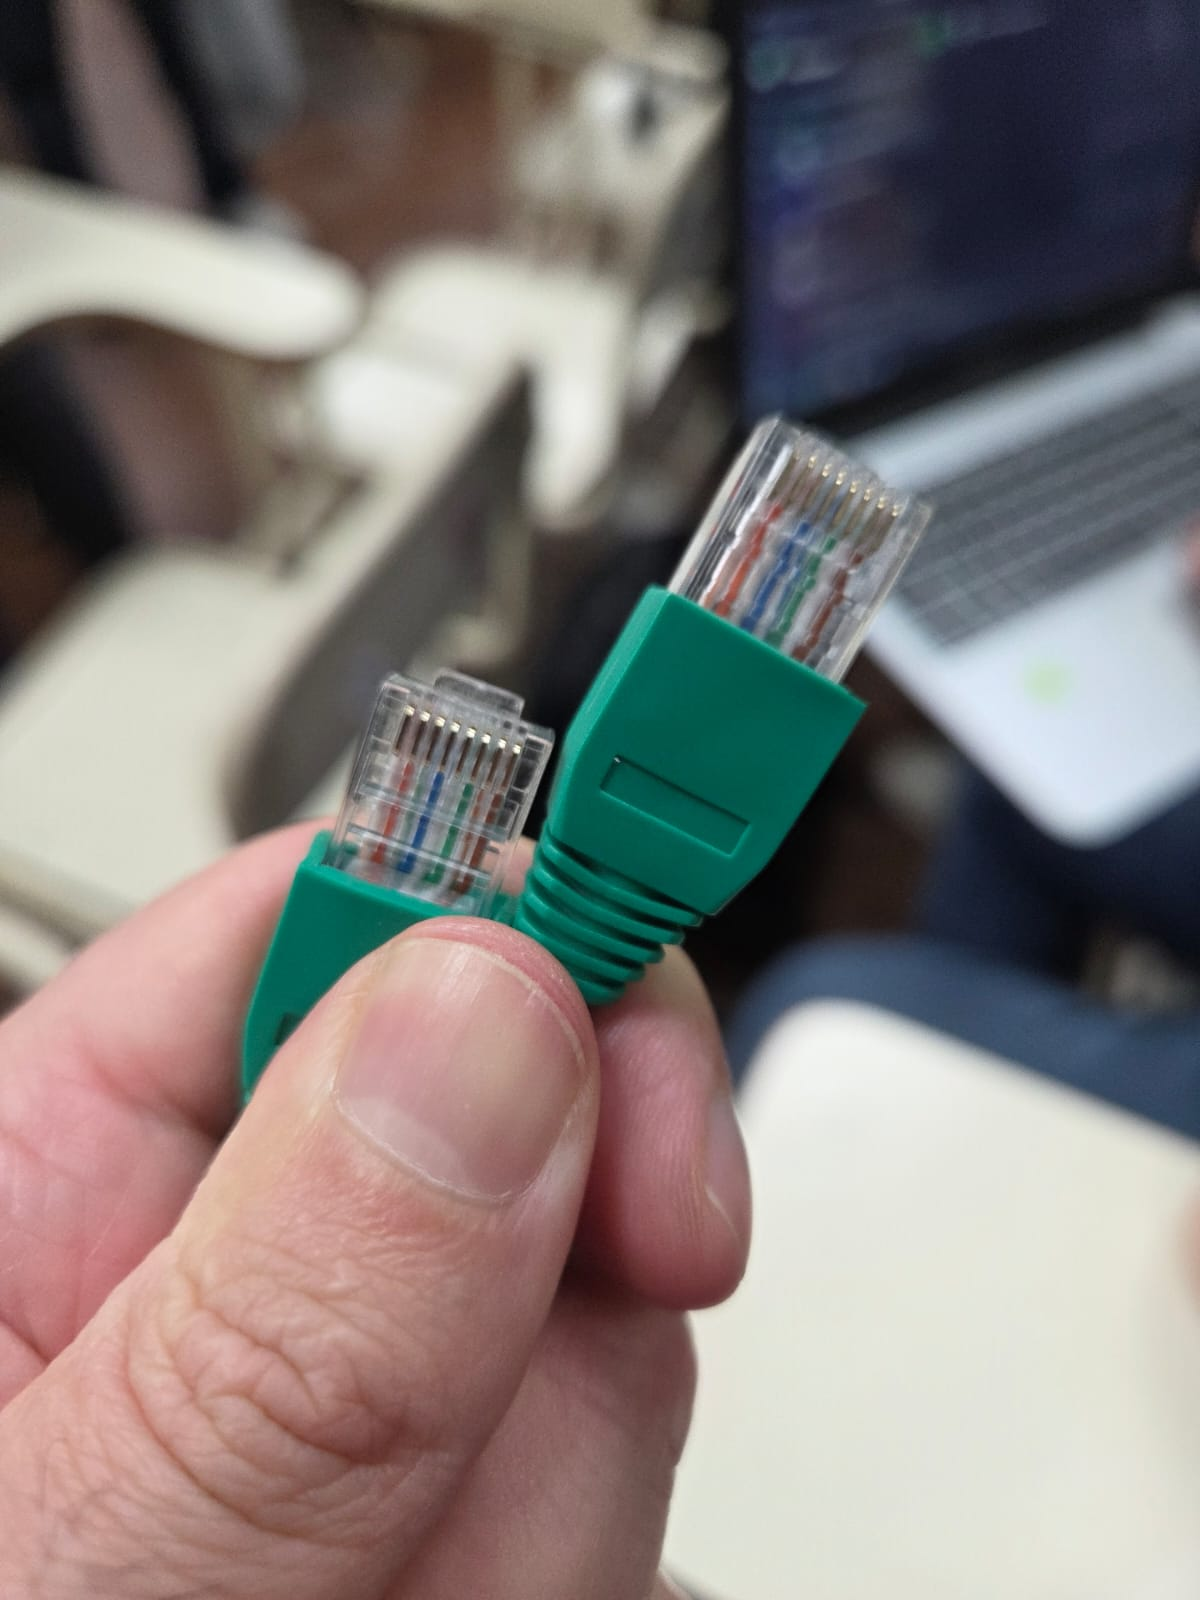
\includegraphics[width=0.75\textwidth]
    {cable-netrunners-T568B.jpeg}
    \caption{Cable Ethernet armado por nuestro grupo con la
    disposición T568B en ambos extremos.}
    \label{fig:cable-t568b}
\end{figure}

\subsection*{Inspección visual del cable del grupo Auracast}

Intercambiamos nuestro cable con el del grupo Auracast para realizar
una inspección visual y verificar su construcción. El grupo
Auracast había utilizado el estándar T568A en ambos extremos, por lo que
también se trataba de un cable directo.

Durante la inspección revisamos la disposición de los
conductores y el armado de los conectores. Los conductores de
cobre estaban correctamente ordenados y asentados en la ficha,
y el cable funcionó correctamente durante la prueba realizada.
Sin embargo, observamos que el plástico de la ficha parecía haber
recibido poca presión durante el crimpado. Por ello, no sujetaba
correctamente la cubierta externa del cable, que podía moverse y
daba la apariencia de estar flojo.

\begin{figure}[H]
    \centering
    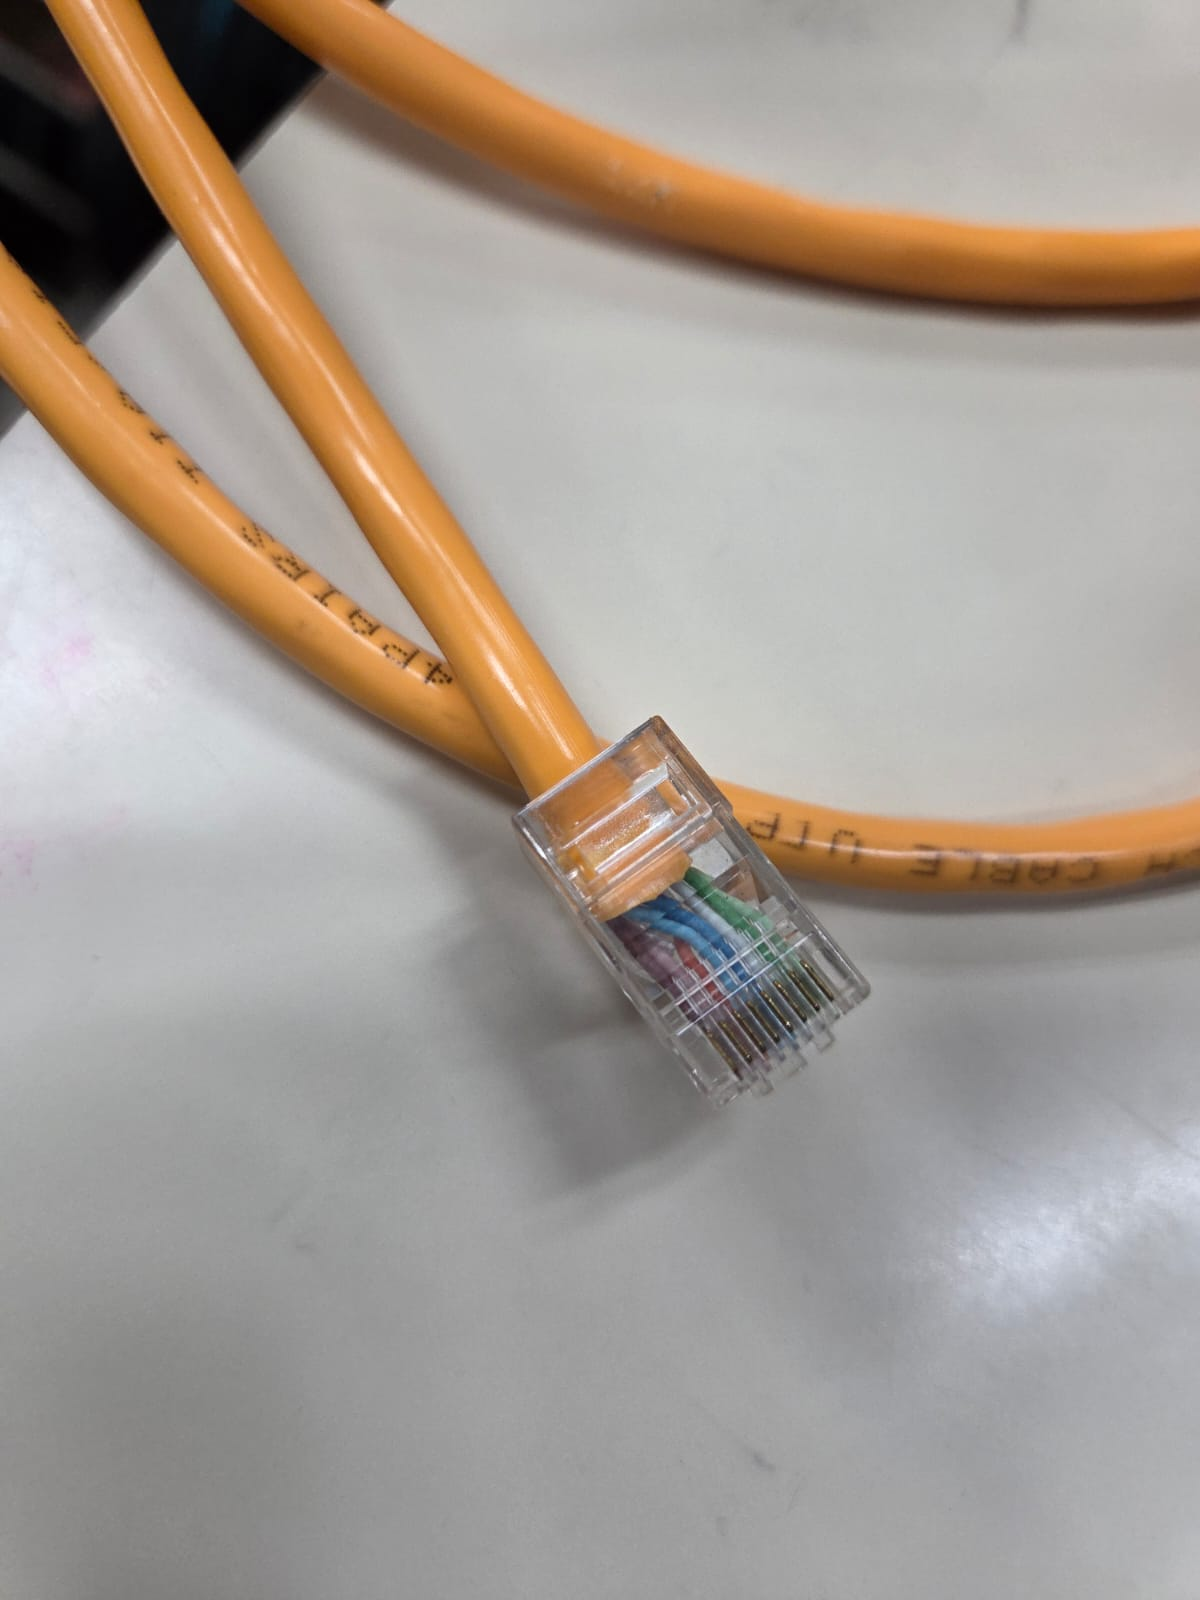
\includegraphics[width=0.75\textwidth]
    {cable-auracast-T568A.jpeg}
    \caption{Cable del grupo Auracast, armado con la disposición
    T568A en ambos extremos.}
    \label{fig:cable-t568a}
\end{figure}

\begin{figure}[H]
    \centering
    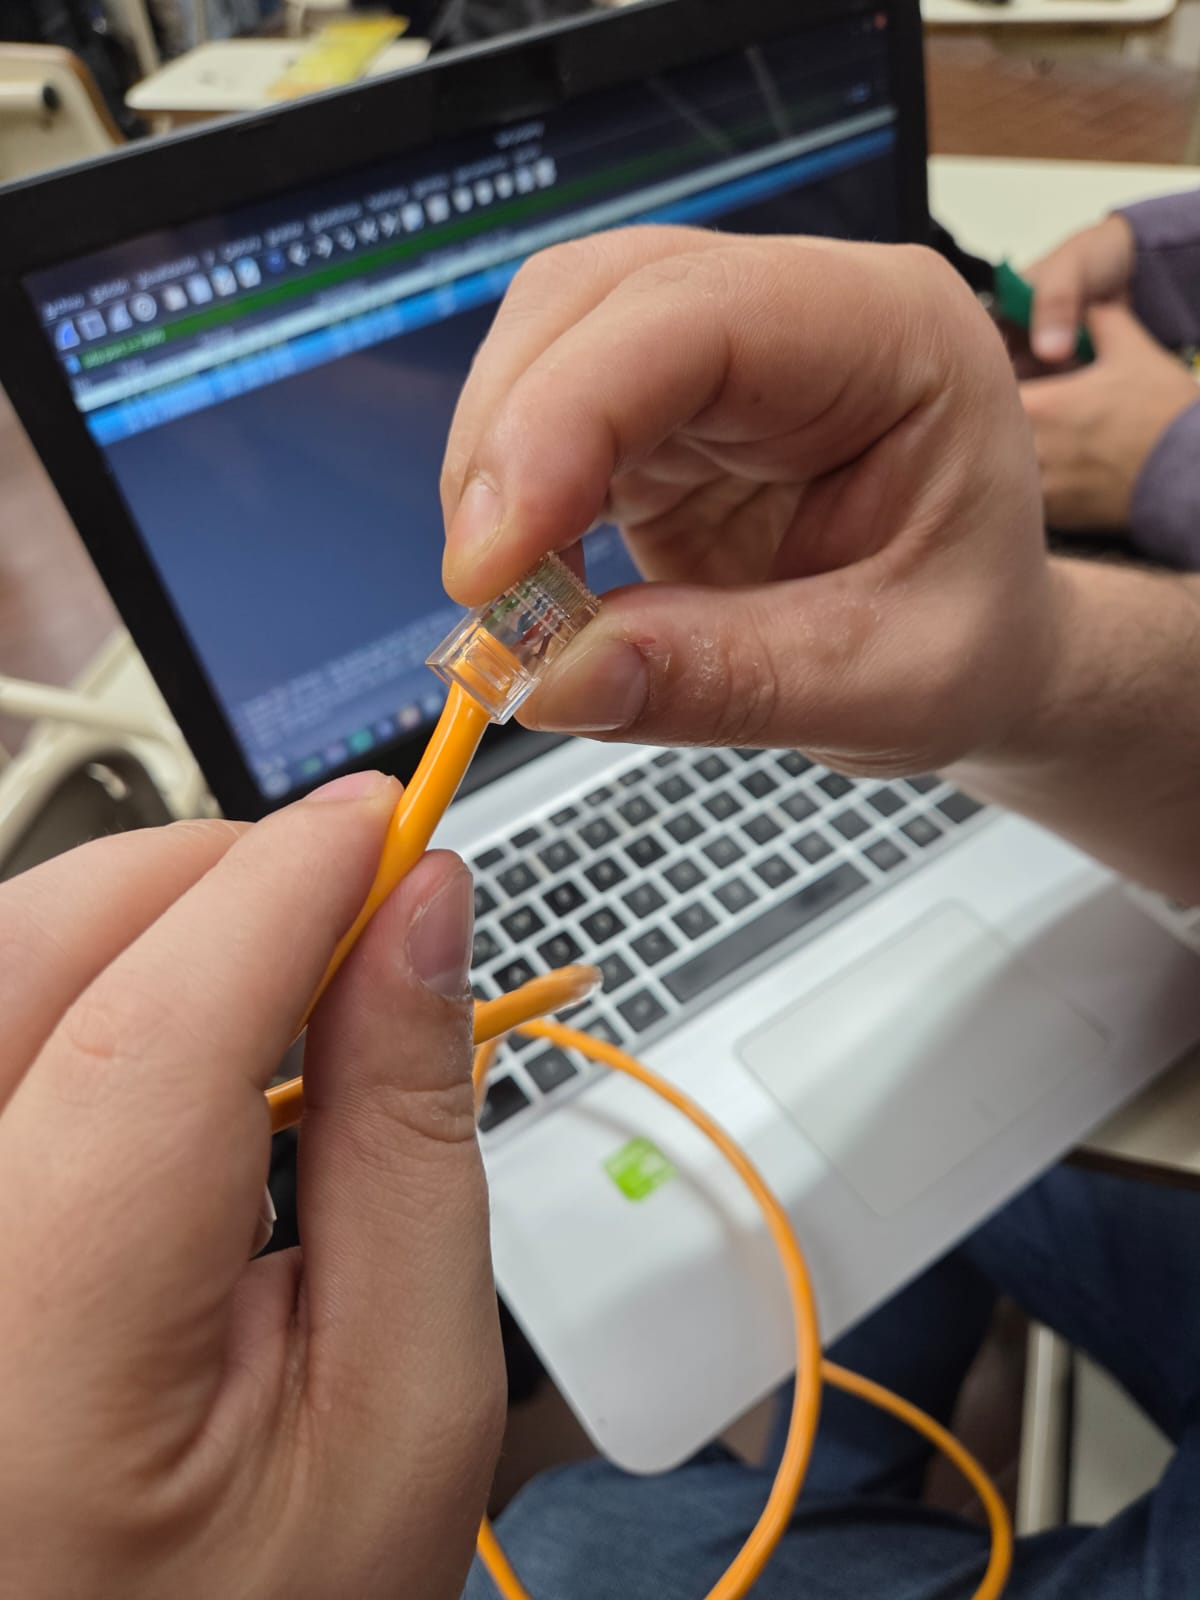
\includegraphics[width=0.45\textwidth]
    {WhatsApp Image 2026-10-15 at 20.12.41.jpeg}
    \caption{Detalle de la ficha del cable Auracast: los conductores
    están correctamente armados, pero el retenedor plástico no
    presiona adecuadamente la cubierta externa del cable.}
    \label{fig:cable-auracast-retenedor}
\end{figure}

\subsection*{Verificación eléctrica mediante tester}

Una vez terminado el armado, verificamos nuestro cable con
un tester de cables Ethernet. Durante la prueba se iluminaron
los ocho indicadores, correspondientes a los pines del 1 al 8,
en secuencia: comenzó por el pin 1, avanzó hasta el pin 8 y
volvió a empezar.

El resultado indicó continuidad en los ocho conductores según
la comprobación realizada con el instrumento.

\section*{Parte 2: Equipamiento físico, verificación y utilización de equipos de red y generación de tráfico.}

\subsection*{Configuración de la LAN y prueba de tráfico UDP}

Configuramos manualmente la interfaz de red de la PC del grupo con
la dirección IPv4 \texttt{192.168.9.245} y la máscara
\texttt{255.255.255.0}, por lo que las PCs participantes quedaron
en la red \texttt{192.168.9.0/24}. La otra PC utilizada durante las
pruebas tenía la dirección \texttt{192.168.9.244}.

La configuración mostraba \texttt{192.168.9.0} como gateway. Esta
dirección identifica la red y no una interfaz utilizable como gateway;
además, no era necesaria para la comunicación entre equipos de la
misma subred. Las transferencias locales se realizaron correctamente
porque ambas direcciones pertenecían a \texttt{192.168.9.0/24}.

\begin{figure}[H]
    \centering
    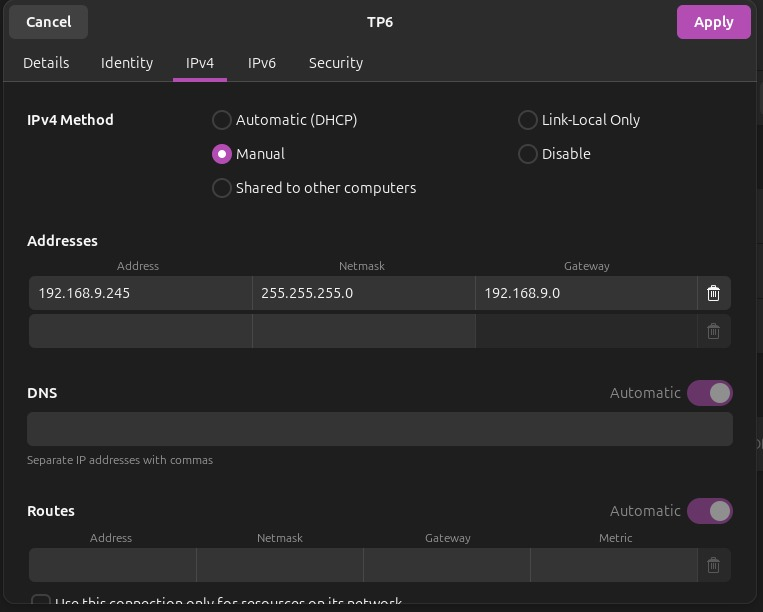
\includegraphics[width=0.7\textwidth]
    {configuracion-ipv4-manual.jpeg}
    \caption{Configuración manual de la interfaz IPv4 de la PC del grupo.}
    \label{fig:ipv4-manual-tp6}
\end{figure}

Verificamos la conectividad con la PC del grupo Auracast mediante
\texttt{ping} a la dirección \texttt{192.168.9.244}. Se recibieron
tres respuestas ICMP consecutivas, con tiempos inferiores a un
milisegundo, lo que confirmó la comunicación entre ambas PCs.

\begin{figure}[H]
    \centering
    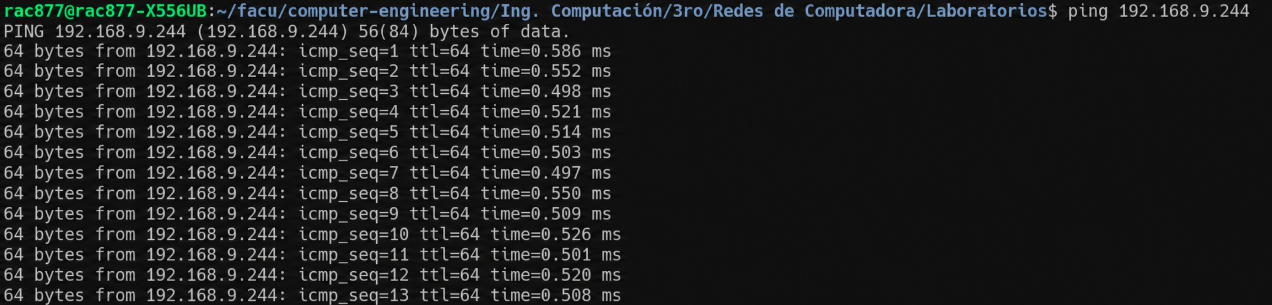
\includegraphics[width=\textwidth]
    {ping-auracast.png}
    \caption{Respuestas ICMP obtenidas al ejecutar \texttt{ping} a la
    PC del grupo Auracast.}
    \label{fig:ping-auracast-tp6}
\end{figure}

Para probar UDP utilizamos \texttt{ncat}. En la PC receptora se
ejecutó \texttt{nc -u -l 5000}; desde la otra PC se enviaron mensajes
al puerto \texttt{5000} de la dirección \texttt{192.168.9.245}. Se
intercambiaron mensajes en ambos sentidos entre los grupos NetRunners
y Auracast.

\begin{figure}[H]
    \centering
    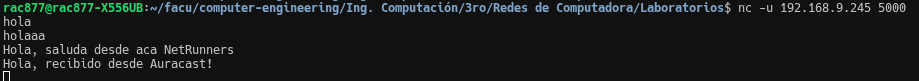
\includegraphics[width=0.7\textwidth]
    {ncat-recepcion.png}
    \caption{Mensajes UDP recibidos por NetRunners mediante \texttt{ncat}.}
    \label{fig:ncat-recepcion-tp6}
\end{figure}

Capturamos el tráfico con Wireshark aplicando el filtro
\texttt{udp.port == 5000}. Se observan datagramas UDP desde
\texttt{192.168.9.244} hacia \texttt{192.168.9.245} y respuestas en
sentido inverso. También se registra un mensaje ICMP
\emph{Destination unreachable (Port unreachable)} al enviar un
datagrama cuando el puerto receptor no estaba disponible.

\begin{figure}[H]
    \centering
    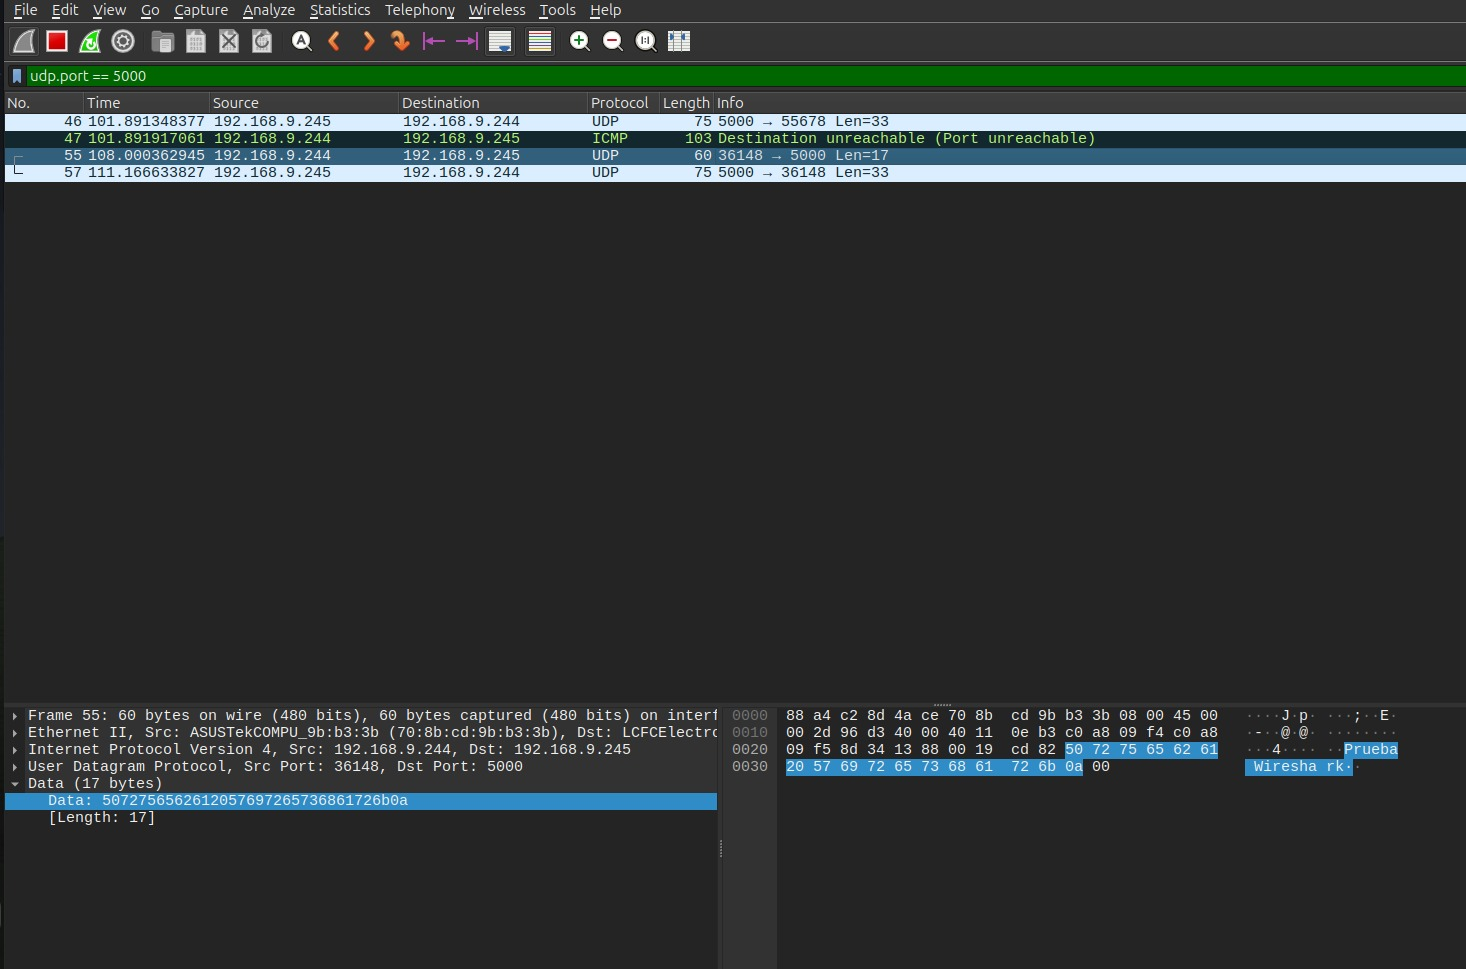
\includegraphics[width=0.9\textwidth]
    {wireshark-udp.jpeg}
    \caption{Captura de Wireshark de los datagramas UDP intercambiados
    por el puerto 5000.}
    \label{fig:wireshark-udp-tp6}
\end{figure}

\begin{enumerate}[label=\alph*)]
    \item No se observa un procedimiento de establecimiento de conexión
    antes del envío de datos, ya que UDP es no orientado a conexión.
    \item UDP no posee un mecanismo de confirmación de recepción
    equivalente a los ACK de TCP.
    \item Si el receptor UDP no está ejecutándose, el datagrama no es
    entregado a una aplicación. En esta prueba se observó la respuesta
    ICMP \emph{Destination unreachable (Port unreachable)}.
    \item UDP no garantiza ni la entrega ni el orden de los mensajes;
    la red puede perderlos, duplicarlos o entregarlos fuera de orden.
    \item Entre las aplicaciones que usan UDP se encuentran DNS, DHCP,
    streaming en tiempo real, videollamadas y juegos en línea. Priorizan
    baja latencia y, cuando hace falta, resuelven pérdidas u orden en la
    propia aplicación.
\end{enumerate}

\subsection*{Desarrollar un pequeño servidor}
  \begin{enumerate}
    \item
    En una de las PC de la LAN creamos el directorio y agregamos tres archivos de diferentes tipos (.txt, .pdf y .jpg) para luego levantar el servidor web.
  
    \begin{figure}[H]
          \centering
          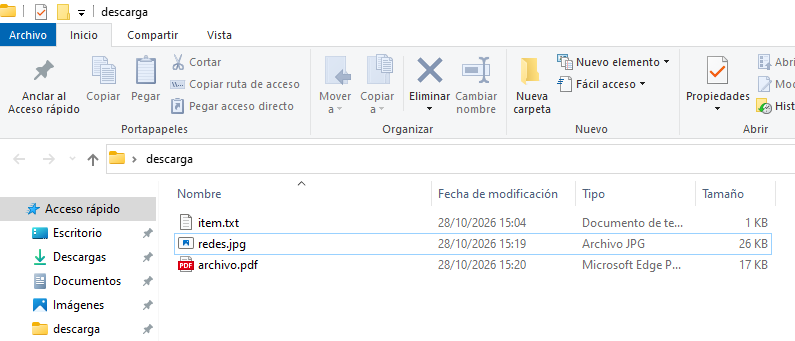
\includegraphics[width=\linewidth]{directory.png}
          \caption{Captura de pantalla del directorio creado.}
          \label{fig:captura_directory}
    \end{figure}


    \item
    Desde la otra PC de la LAN, abrimos un navegador web y accedemos al servidor web, verificando que se pueda acceder a los archivos creados y descargando el archivo "archivo.pdf".

    \begin{figure}[H]
          \centering
          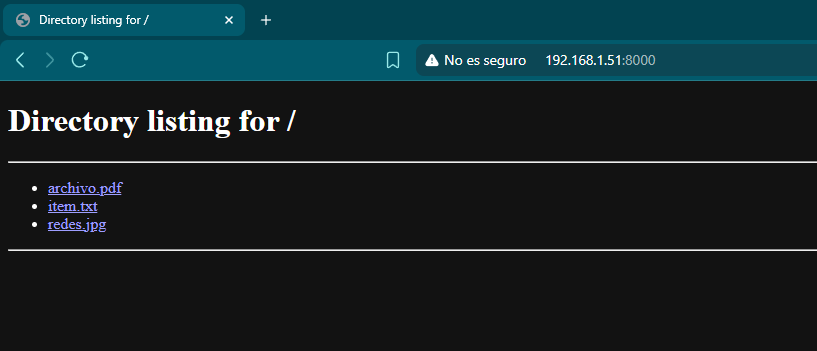
\includegraphics[width=\linewidth]{browser.png}
          \caption{Captura de pantalla del navegador web accediendo al servidor web.}
          \label{fig:captura_browser}
    \end{figure}

    \begin{figure}[H]
          \centering
          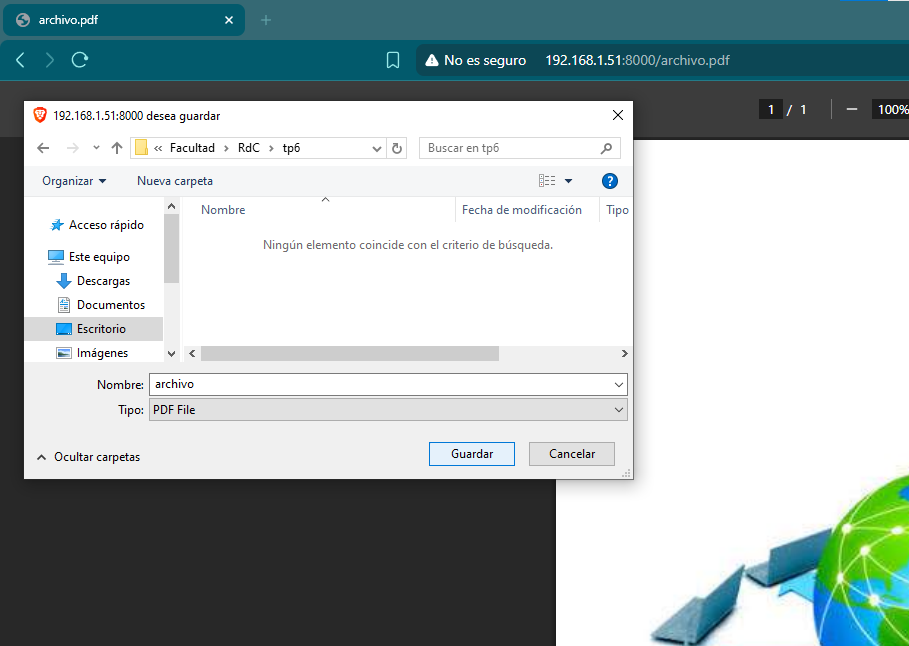
\includegraphics[width=\linewidth]{download.png}
          \caption{Captura de pantalla de la descarga del archivo.}
          \label{fig:captura_download}
    \end{figure}

    \item

    Repetimos la transferencia usando ahora curl mediante un terminal:

    \begin{figure}[H]
          \centering
          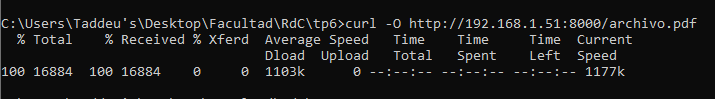
\includegraphics[width=\linewidth]{download_curl.png}
          \caption{Captura de pantalla de la transferencia con curl.}
          \label{fig:captura_curl}
    \end{figure}

    \item
    Capturamos el tráfico generado por la transferencia de archivos con Wireshark. Observamos que se trató de una transferencia HTTP mediante una petición GET.
    \begin{figure}[H]
          \centering
          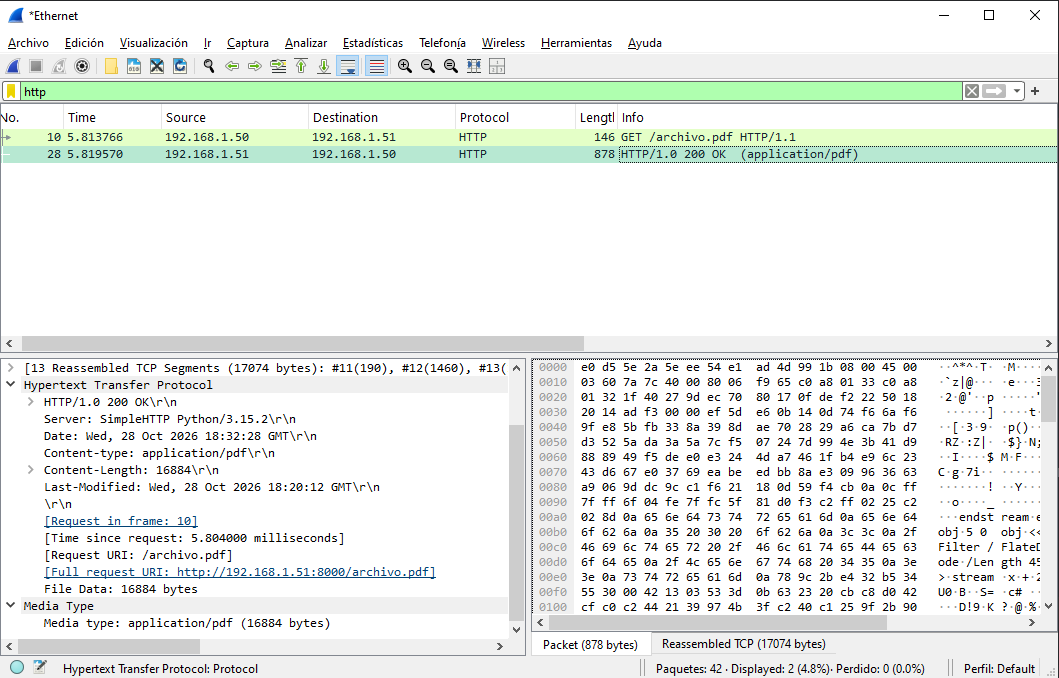
\includegraphics[width=\linewidth]{wireshark.png}
          \caption{Captura de pantalla de la captura de tráfico con Wireshark.}
          \label{fig:captura_wireshark}
    \end{figure}
  \end{enumerate}

\end{document}
